% !TEX root = ../thesis.tex
\section{Example Interactive Visualizations}
\label{sec:vg:examples}

\vspace{-10pt}

To evaluate the expressivity of our language, we present a range of examples and
demonstrate coverage over Yi~et~al.'s interaction
taxonomy~\cite{yi:understanding}. Yi~et~al. identify seven categories based on
user intent: \emph{select}, to mark items of interest; \emph{connect}, to show
related items; \emph{abstract/elaborate}, to show more or less detail;
\emph{explore}, to examine a different subset of data; \emph{reconfigure}, to
show a different arrangement of data; \emph{filter}, to show something
conditionally; and, \emph{encode}, to use a different visual encoding. It is
important to note that these categories are not mutually exclusive, and an
interaction technique can be classified under several categories. We choose
example interactive visualizations to demonstrate that our model can express
interactions across all seven categories and how, through composition of its
primitives, supports the accretive design of richer interactions.

\begin{figure}[h!]
  \centering
  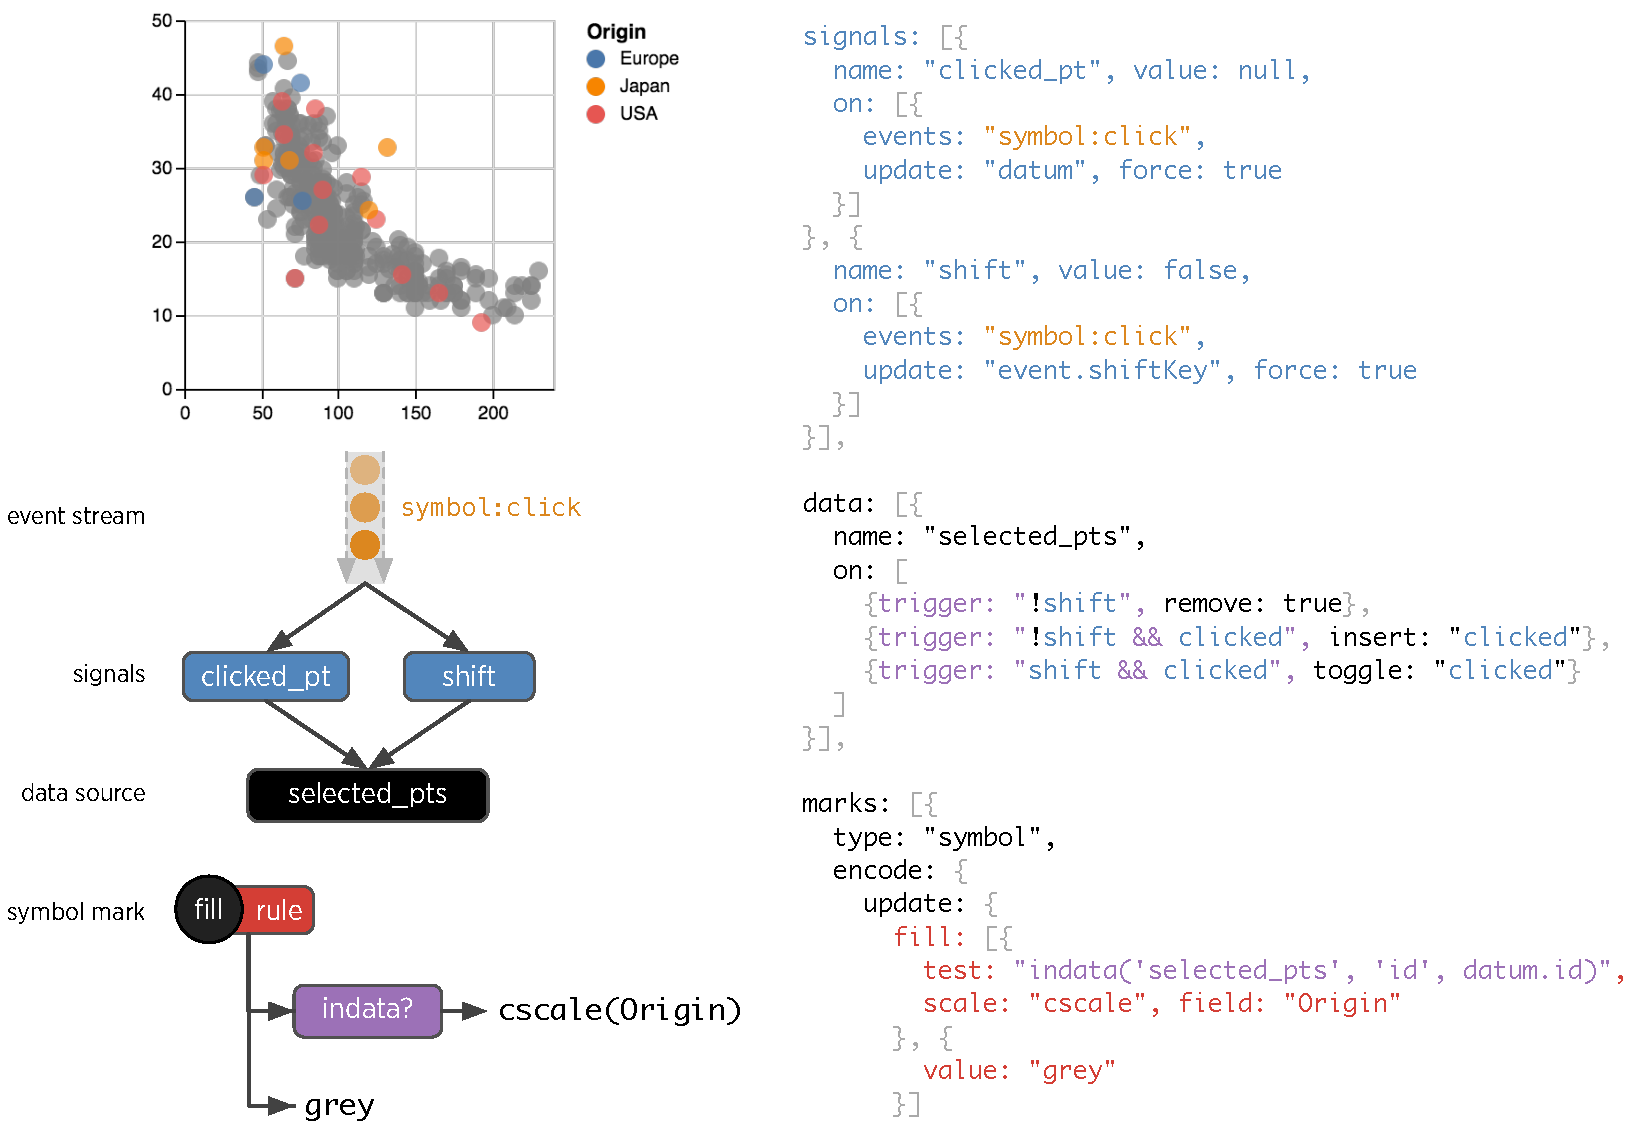
\includegraphics[width=\columnwidth]{shiftClick}
  \caption{Reactive Vega JSON for a click-to-highlight interaction. Signals over
  a click stream feed data transform to toggle values in a data source. A
  production rule uses a predicate to set marks' fill color.}
  \label{fig:vg:shiftClick}
\end{figure}

\subsection{Selection: Click/Shift-Click and Brushing}

\vspace{-7pt}

\Cref{fig:vg:shiftClick} provides a snippet of Reactive Vega JSON for a
click-to-highlight interaction. Signals constructed over a click stream feed
data transforms that toggle values in the \texttt{selected\_pts} data source. An
intensional predicate tests for the shift key. If it is not pressed, the data
source is cleared prior to inserting the clicked values. A production rule sets
the fill color of selected points using an extensional predicate.

Similarly, \cref{fig:vg:brush} demonstrates the Reactive Vega JSON necessary to
enable brush selections. Signals are registered to capture the start and end
positions of the brush, by default \texttt{mousedown} and \texttt{[mousedown,
mouseup] > mousemove}, respectively. Scale inversions are invoked to calculate
the data extents of the brush, which are used to define an intensional predicate
to express the brushed data range. As before, the predicate is used within a
production rule to set the fill color of selected points.

\begin{figure}[h!]
  \centering
  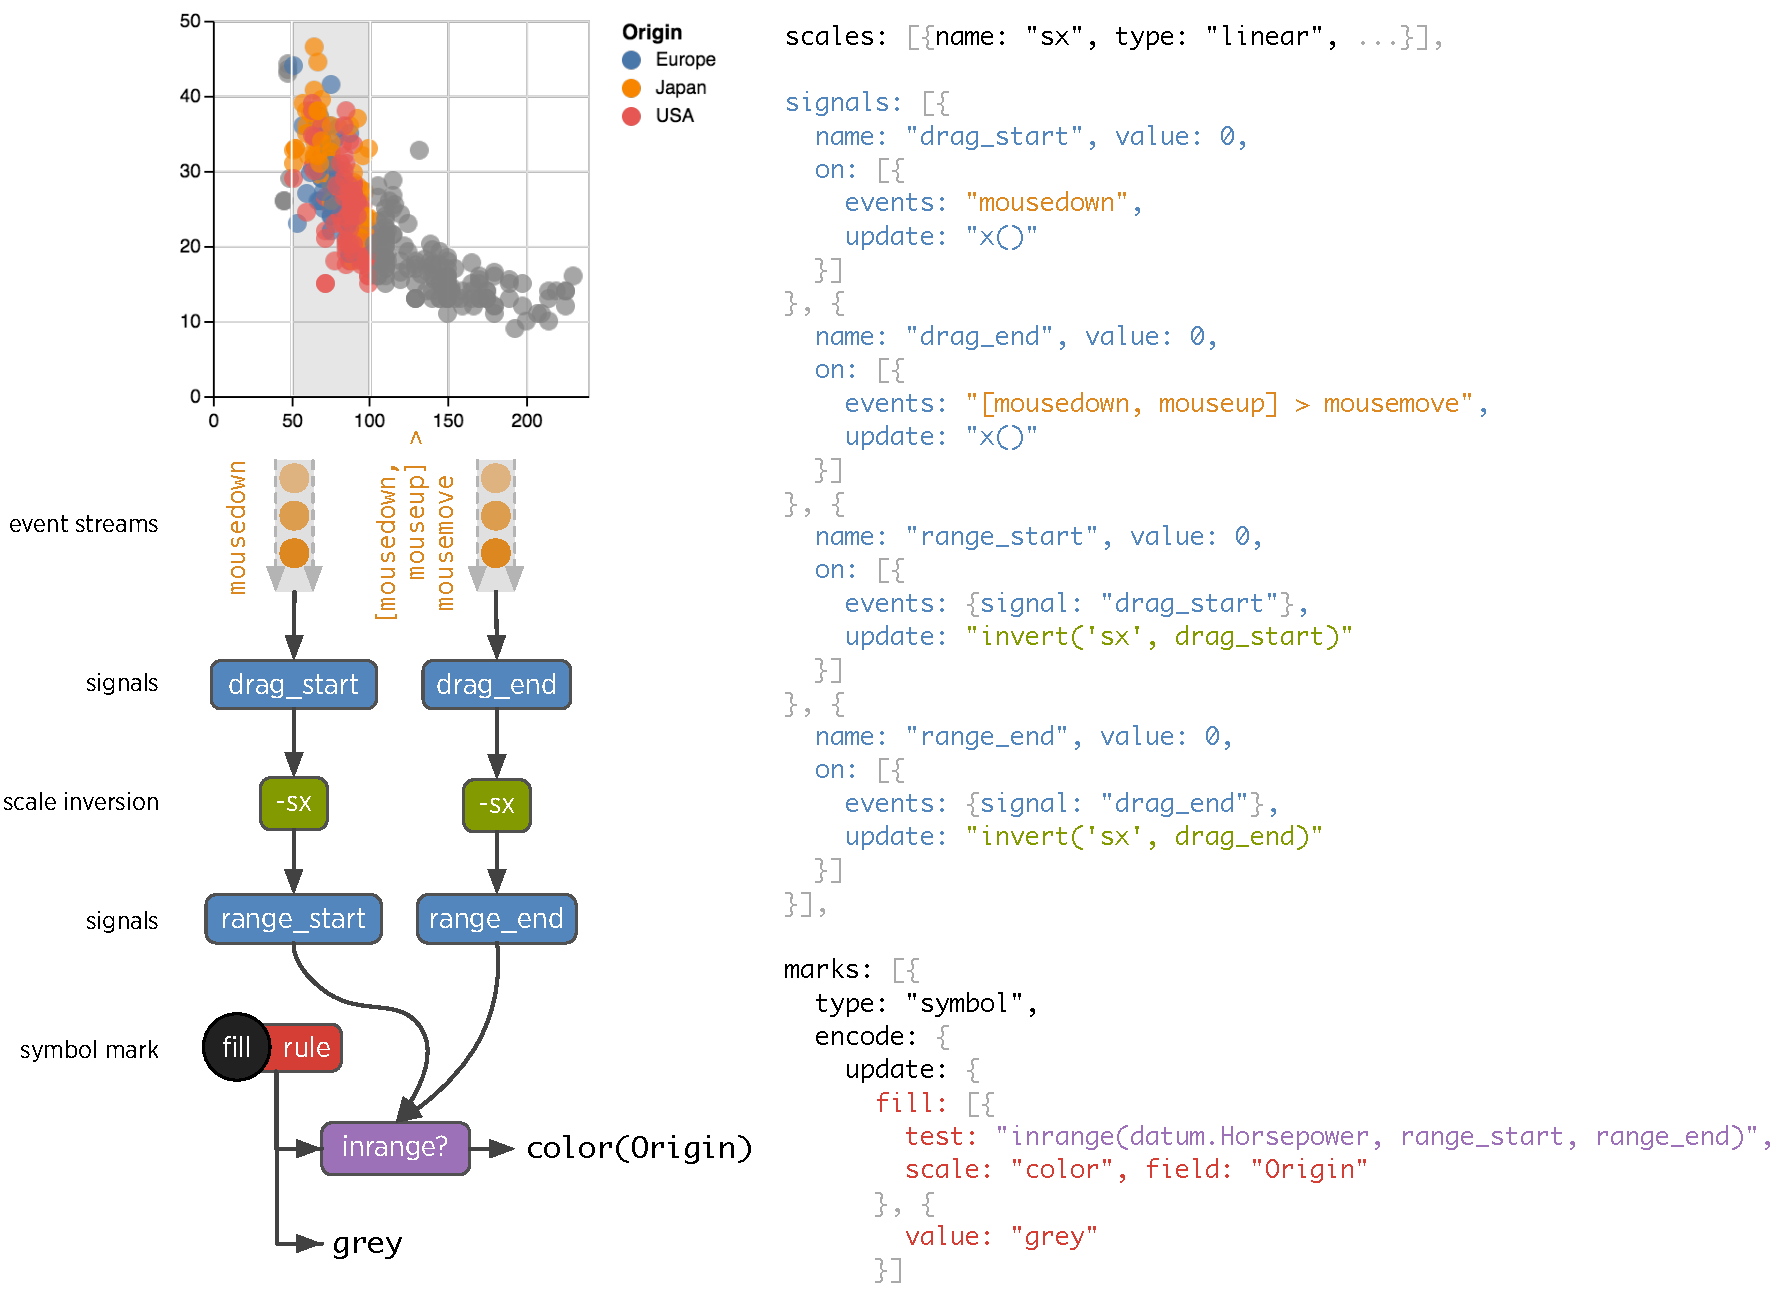
\includegraphics[width=0.9\columnwidth]{brush}
  \caption{A JSON snippet for one-dimensional brushing. Signals over drag
  events are inverted through the x-scale to construct a data query over the
  \texttt{Horsepower} field.}
  \label{fig:vg:brush}
\end{figure}

\begin{figure}[h!]
  \centering
  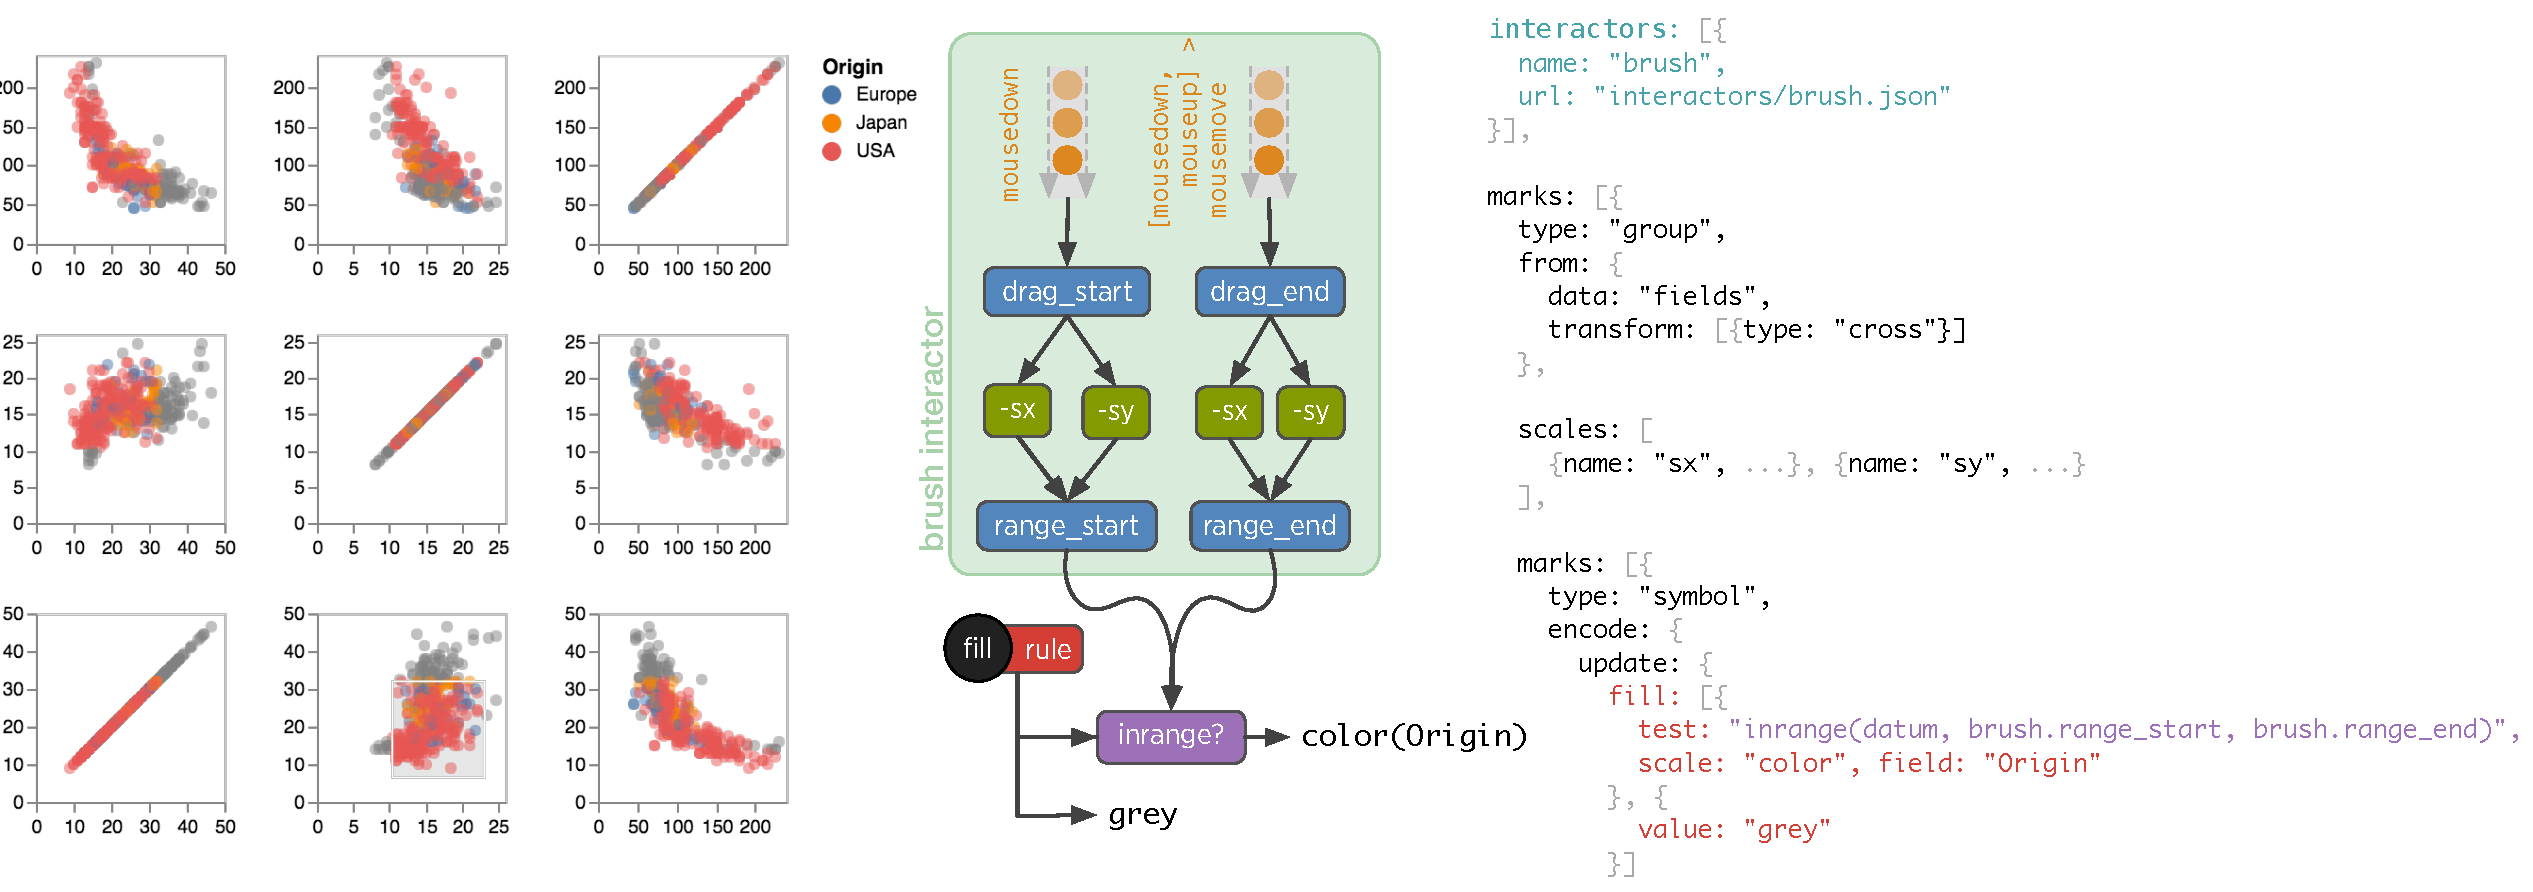
\includegraphics[width=\columnwidth]{splomInteractor}
  \caption{We can extract the brushing interaction from \cref{fig:vg:brush}
  into a standalone interactor, and reapply it to a scatterplot matrix to
  perform brushing \& linking.}
  \label{fig:vg:splomInteractor}
\end{figure}

\subsection{Connect: Brushing \& Linking}

\vspace{-7pt}

\begin{wrapfigure}{l}{0pt}
  \raisebox{0pt}[\dimexpr\height-0.6\baselineskip\relax]{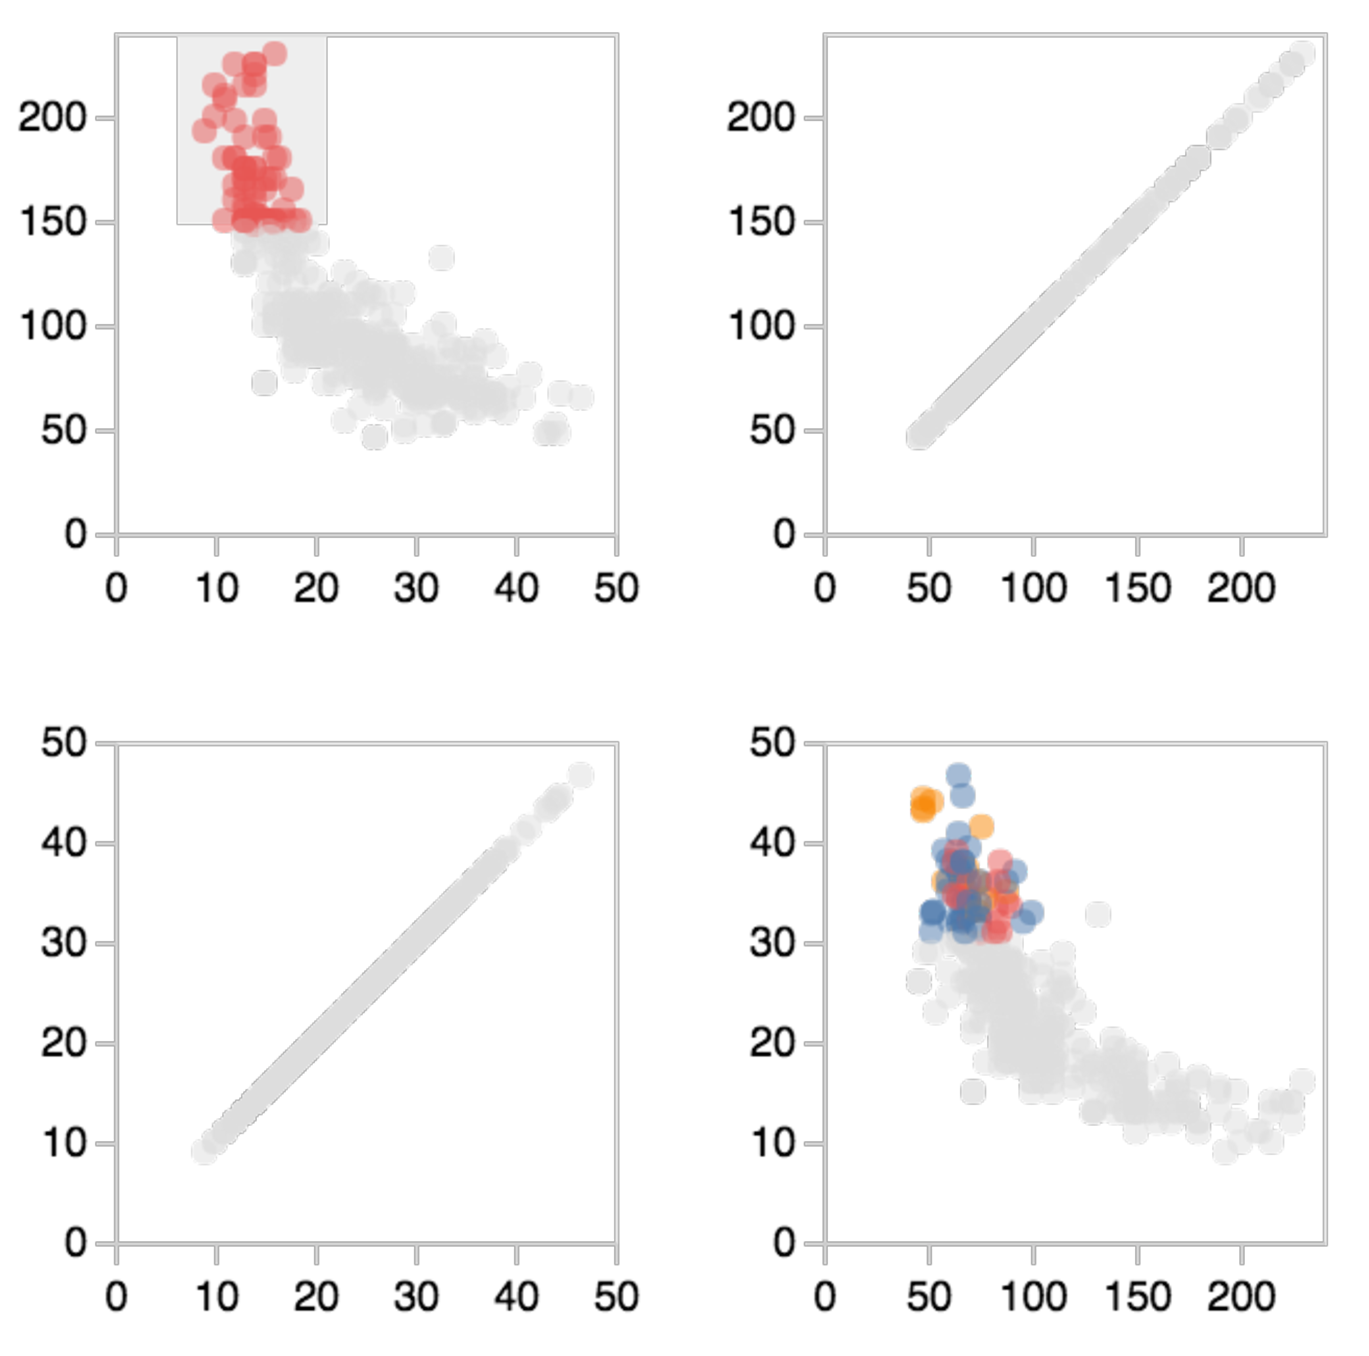
\includegraphics
  [width=0.27\textwidth]{splomPixel}}
\end{wrapfigure}

We can extract the previous interaction into a standalone ``brushing''
interactor, and then apply it to brush \& link a scatterplot matrix as shown in
\cref{fig:vg:splomInteractor}. Each cell of the matrix is an instance of a group
mark with its own coordinate space. The plotting symbol and spatial scale
functions are defined within these groups. Had the interactor's predicates
defined selections over pixel space, the production rule would highlight points
that fall along the same horizontal and vertical pixel regions\,---\,for
example, in the inset figure, brushing over red points would highlight no or
blue points in the other cells. Instead, the interactor uses scale inversions to
lift the predicate to the data domain, and the production rule correctly links
brushed points across scatterplots.

\vspace{-10pt}

\subsection{Abstract/Elaborate: Overview\,+\,Detail}

\vspace{-7pt}

With our brush interactor, we can also create the overview\,+\,detail
visualization in \cref{fig:vl:scaleInversion}. In this case, brushing is
restricted to the horizontal dimension by overriding the \texttt{height}
property of the interactor's mark, and ignoring the vertical range predicates it
populates. We use the horizontal range predicate with a filter transformation,
to filter points for display in the detail plot. As a user brushes, signals
update the range predicate, which in turn filters points in the data source,
updates scale functions and re-renders the detail view.

\vspace{-10pt}

\subsection{Explore \& Encode: Panning \& Zooming}

\vspace{-7pt}

\begin{figure}[b!]
  \centering
  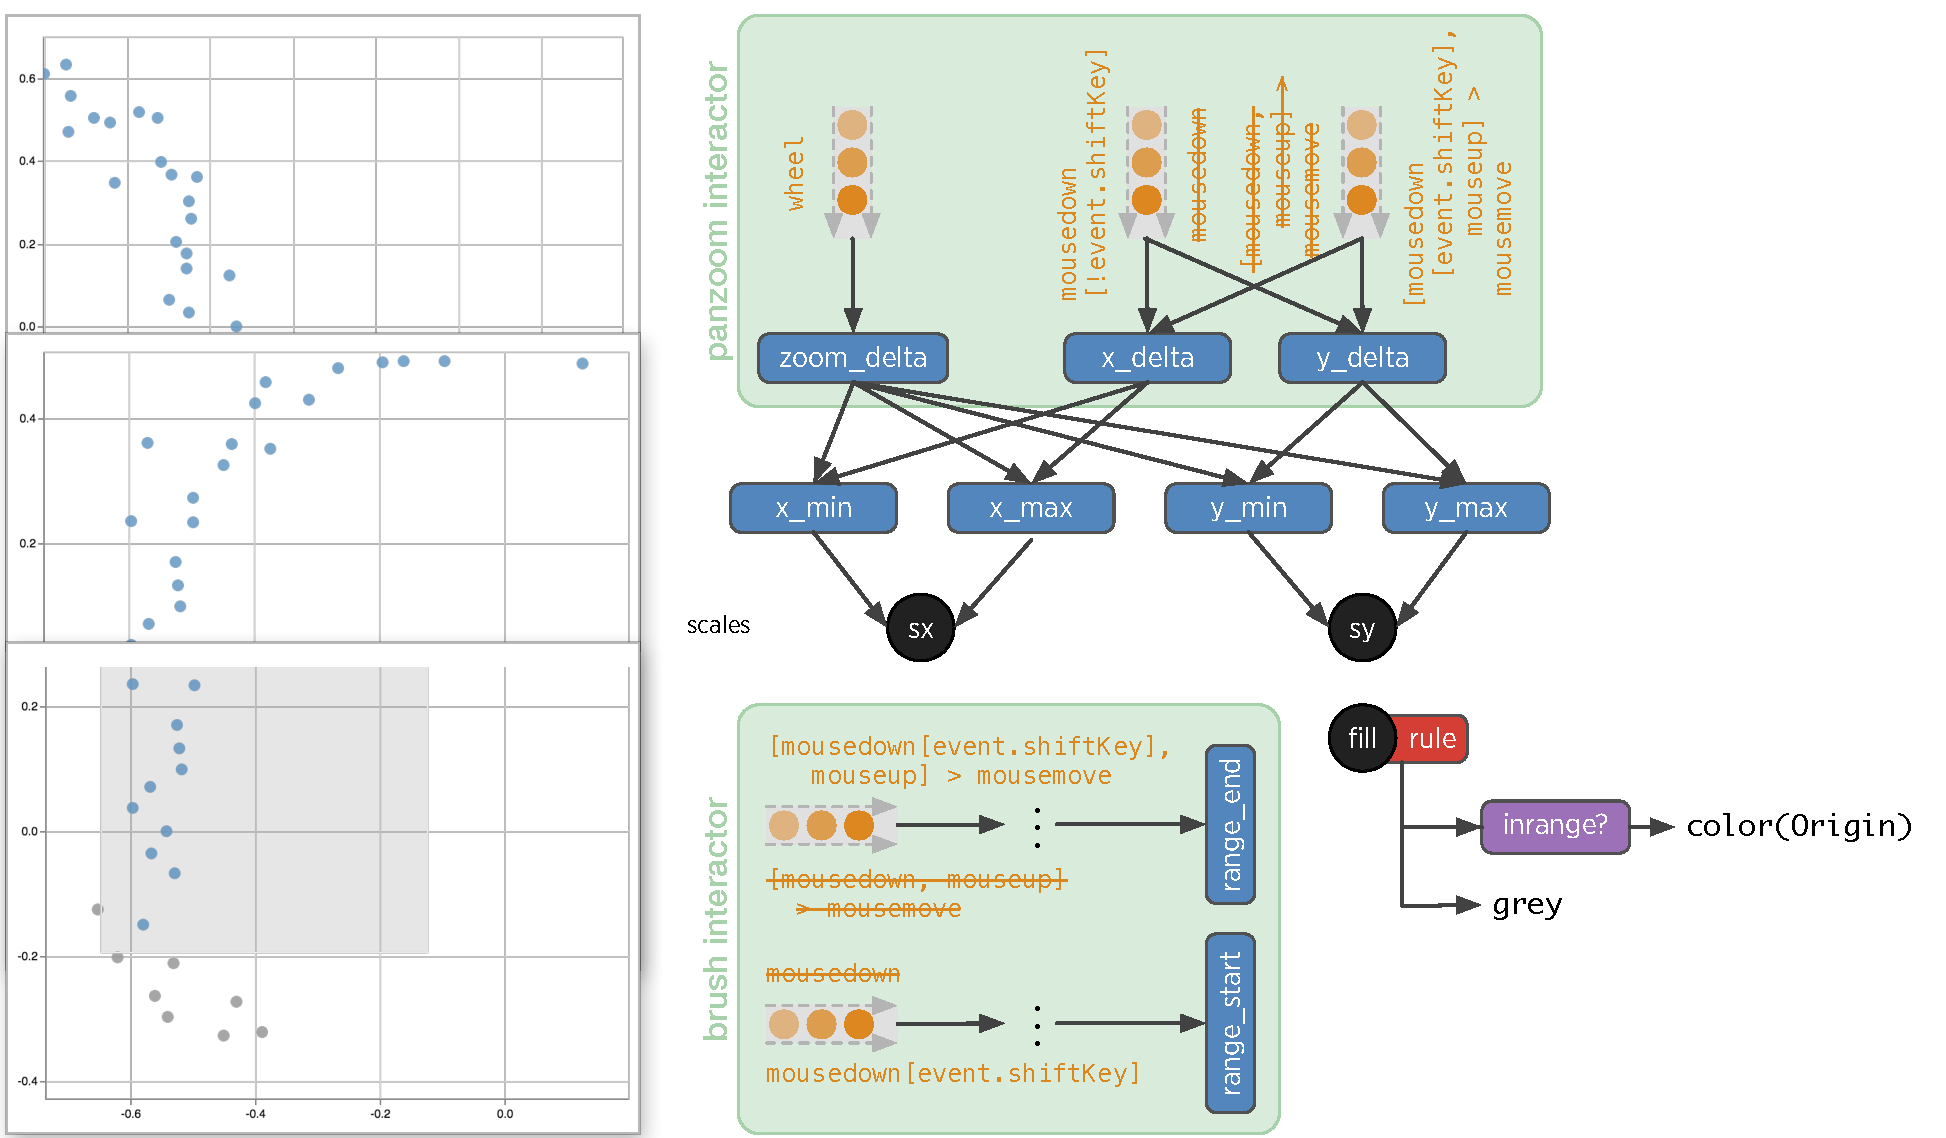
\includegraphics[width=\columnwidth]{panzoom}
  \caption{Panning \& zooming a scatterplot. Brushing is accretively added with
  the brush interactor (\cref{fig:vg:brush,fig:vg:splomInteractor}), and
  conflicts are resolved by rebinding event streams (indicated with
  strikethroughs).}
  \label{fig:vg:panzoom}
\end{figure}

\Cref{fig:vg:panzoom} shows pan and zoom interactions for a scatter plot. By
default, scale functions calculate their domain automatically from a data
source. For this interaction, however, we must parameterize the domain using
reactive signals. For panning, a \texttt{start} signal captures an initial
\texttt{(x,y)} position on \texttt{mousedown}, and subsequent \texttt{pan}
signals calculate a delta on drag (\texttt{[mousedown, mouseup] > mousemove}).
This delta is used to offset the scale domains. Similarly, when \texttt{wheel}
events occur, a \texttt{zoom} signal applies a scale factor to the domains
depending on the zoom direction.

\begin{figure}[t!]
  \centering
  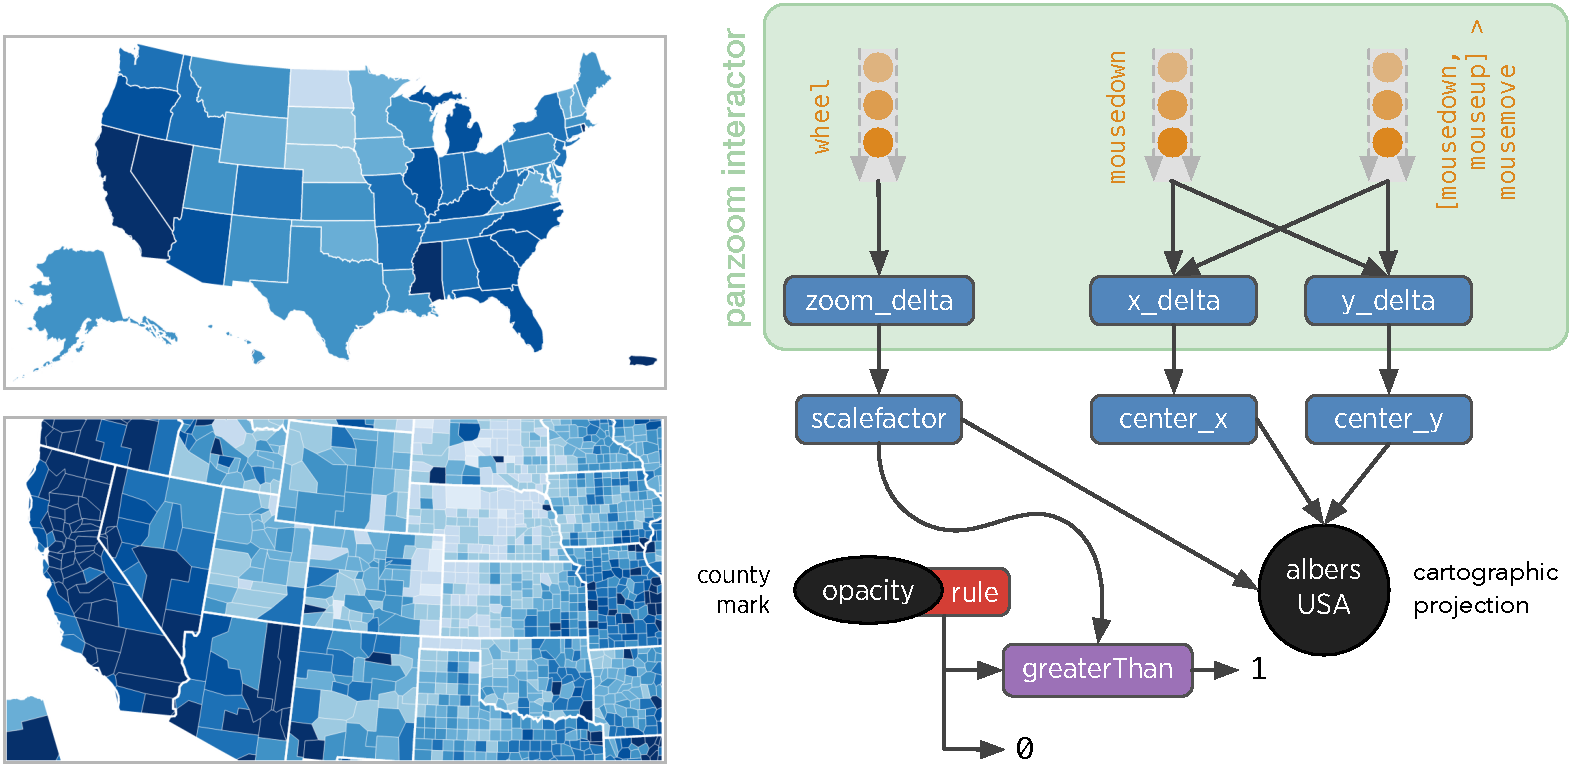
\includegraphics[width=\columnwidth]{semanticZoom}
  \caption{Extracting the pan \& zoom interaction from \cref{fig:vg:panzoom}
  into an interactor, and repurposing it to perform \emph{semantic} zooming on a
  cartographic map. Initially, a choropleth of state-level unemployment in the
  United States is shown. Zooming past a threshold, states break up into
  counties, and show county-level unemployment instead.}
  \label{fig:vg:semanticZoom}
\end{figure}

If we were to also add a brushing interaction to this visualization, a na\"ive
application would yield a conflicting interaction: on drag, both panning and
brushing would occur. One option to resolve this conflict is to begin brushing
only when the shift key is pressed. If we try combining these interactions using
D3~\cite{bostock:d3}, which offers brushing and panning as part of its
interactor typology, specifying this resolution scheme can be onerous.
Additional callbacks must be registered that either instantiate or destroy a
particular interaction depending on the state of the shift key.

With Reactive Vega, the brush and pan signals can be rebound without modifying
the interactor definitions. Instead, we provide alternate source event streams
when instantiating the interactor\,---\,\texttt{mousedown[event.shiftKey]} for
brushing, and\\\texttt{mousedown[!event.shiftKey]} for panning.

Moreover, by extracting panning \& zooming into a standalone interactor, we can
repurpose the behavior to instead trigger semantic zooming~\cite{perlin:pad}, an
\emph{encoding} interaction technique shown in \cref{fig:vg:semanticZoom}. At
the top-level, the visualization shows a choropleth map of state-level
unemployment. After crossing a specified zoom threshold, states subdivide to
show a choropleth map of country-level unemployment. Here, the pan signals drive
the geographic projection's translation and the zoom signals drive the
projection's scale parameter. By default, both maps are drawn with states
overlaying counties. A production rule uses a predicate to test whether the zoom
signal is above a specified threshold; if it is, the state-level map is rendered
transparently, displaying the county-level map underneath it.

\vspace{-10pt}

\subsection{Reconfigure: Index Chart}

\vspace{-7pt}

\begin{figure}[b!]
  \centering
  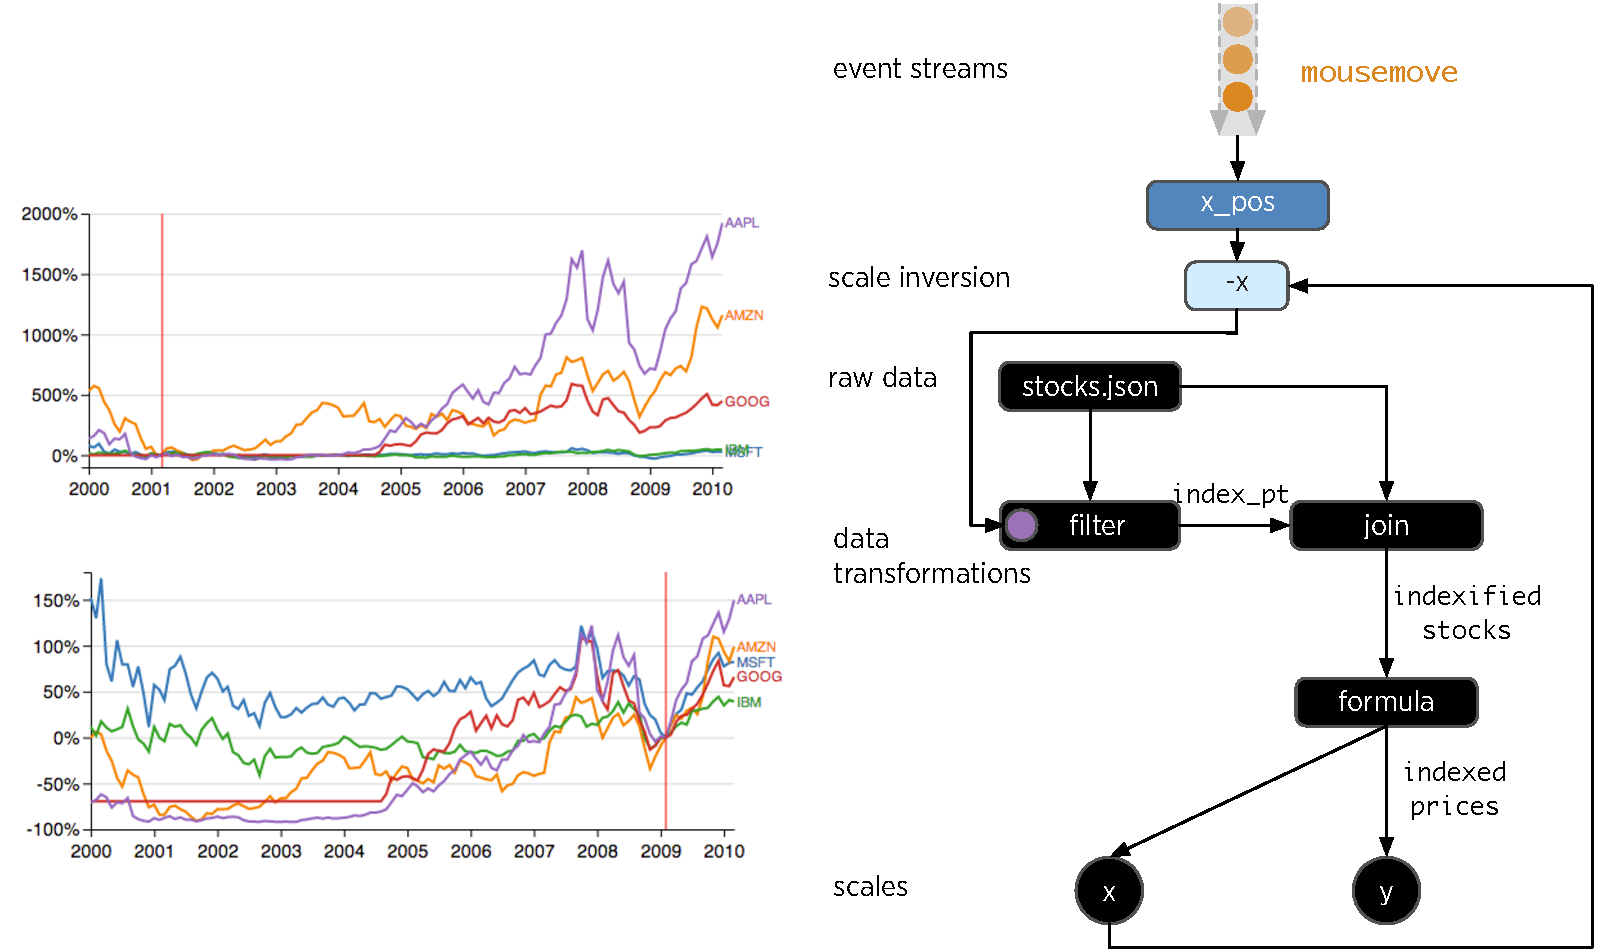
\includegraphics[width=0.89\columnwidth]{indexChart}
  \caption{An index chart shows the percentage changes for time-series data. The
  index point (red vertical line) is determined by the x position of a
  \texttt{mousemove} signal, which filters points using a predicate.}
  \label{fig:vg:indexChart}
\end{figure}

\Cref{fig:vg:indexChart} shows an index chart: a line chart that interactively
normalizes time series to show percentage change based on the current index
point. To calculate the index point, a signal captures the \texttt{x} coordinate
of \texttt{mousemove}events, and drives it through a scale inversion. As it is a
quantitative scale, scale inversion produces a value from a continuous domain
(i.e., any date/time from Jan 1 2000--Dec 31 2010). However, our dataset only
contains stock prices for the start of every month. We use a predicate to ``snap
to'' the closest value for each time series, and use this as our index point.
Using Vega's data transformations, we join the index point against the original
data set and normalize the data values. Scale functions are defined in terms of
the normalized data.

\vspace{-10pt}

\subsection{Reconfigure: Reordering Columns of a Matrix}

\vspace{-7pt}

\begin{wrapfigure}{l}{0pt}
  \raisebox{0pt}[\dimexpr\height-0.6\baselineskip\relax]{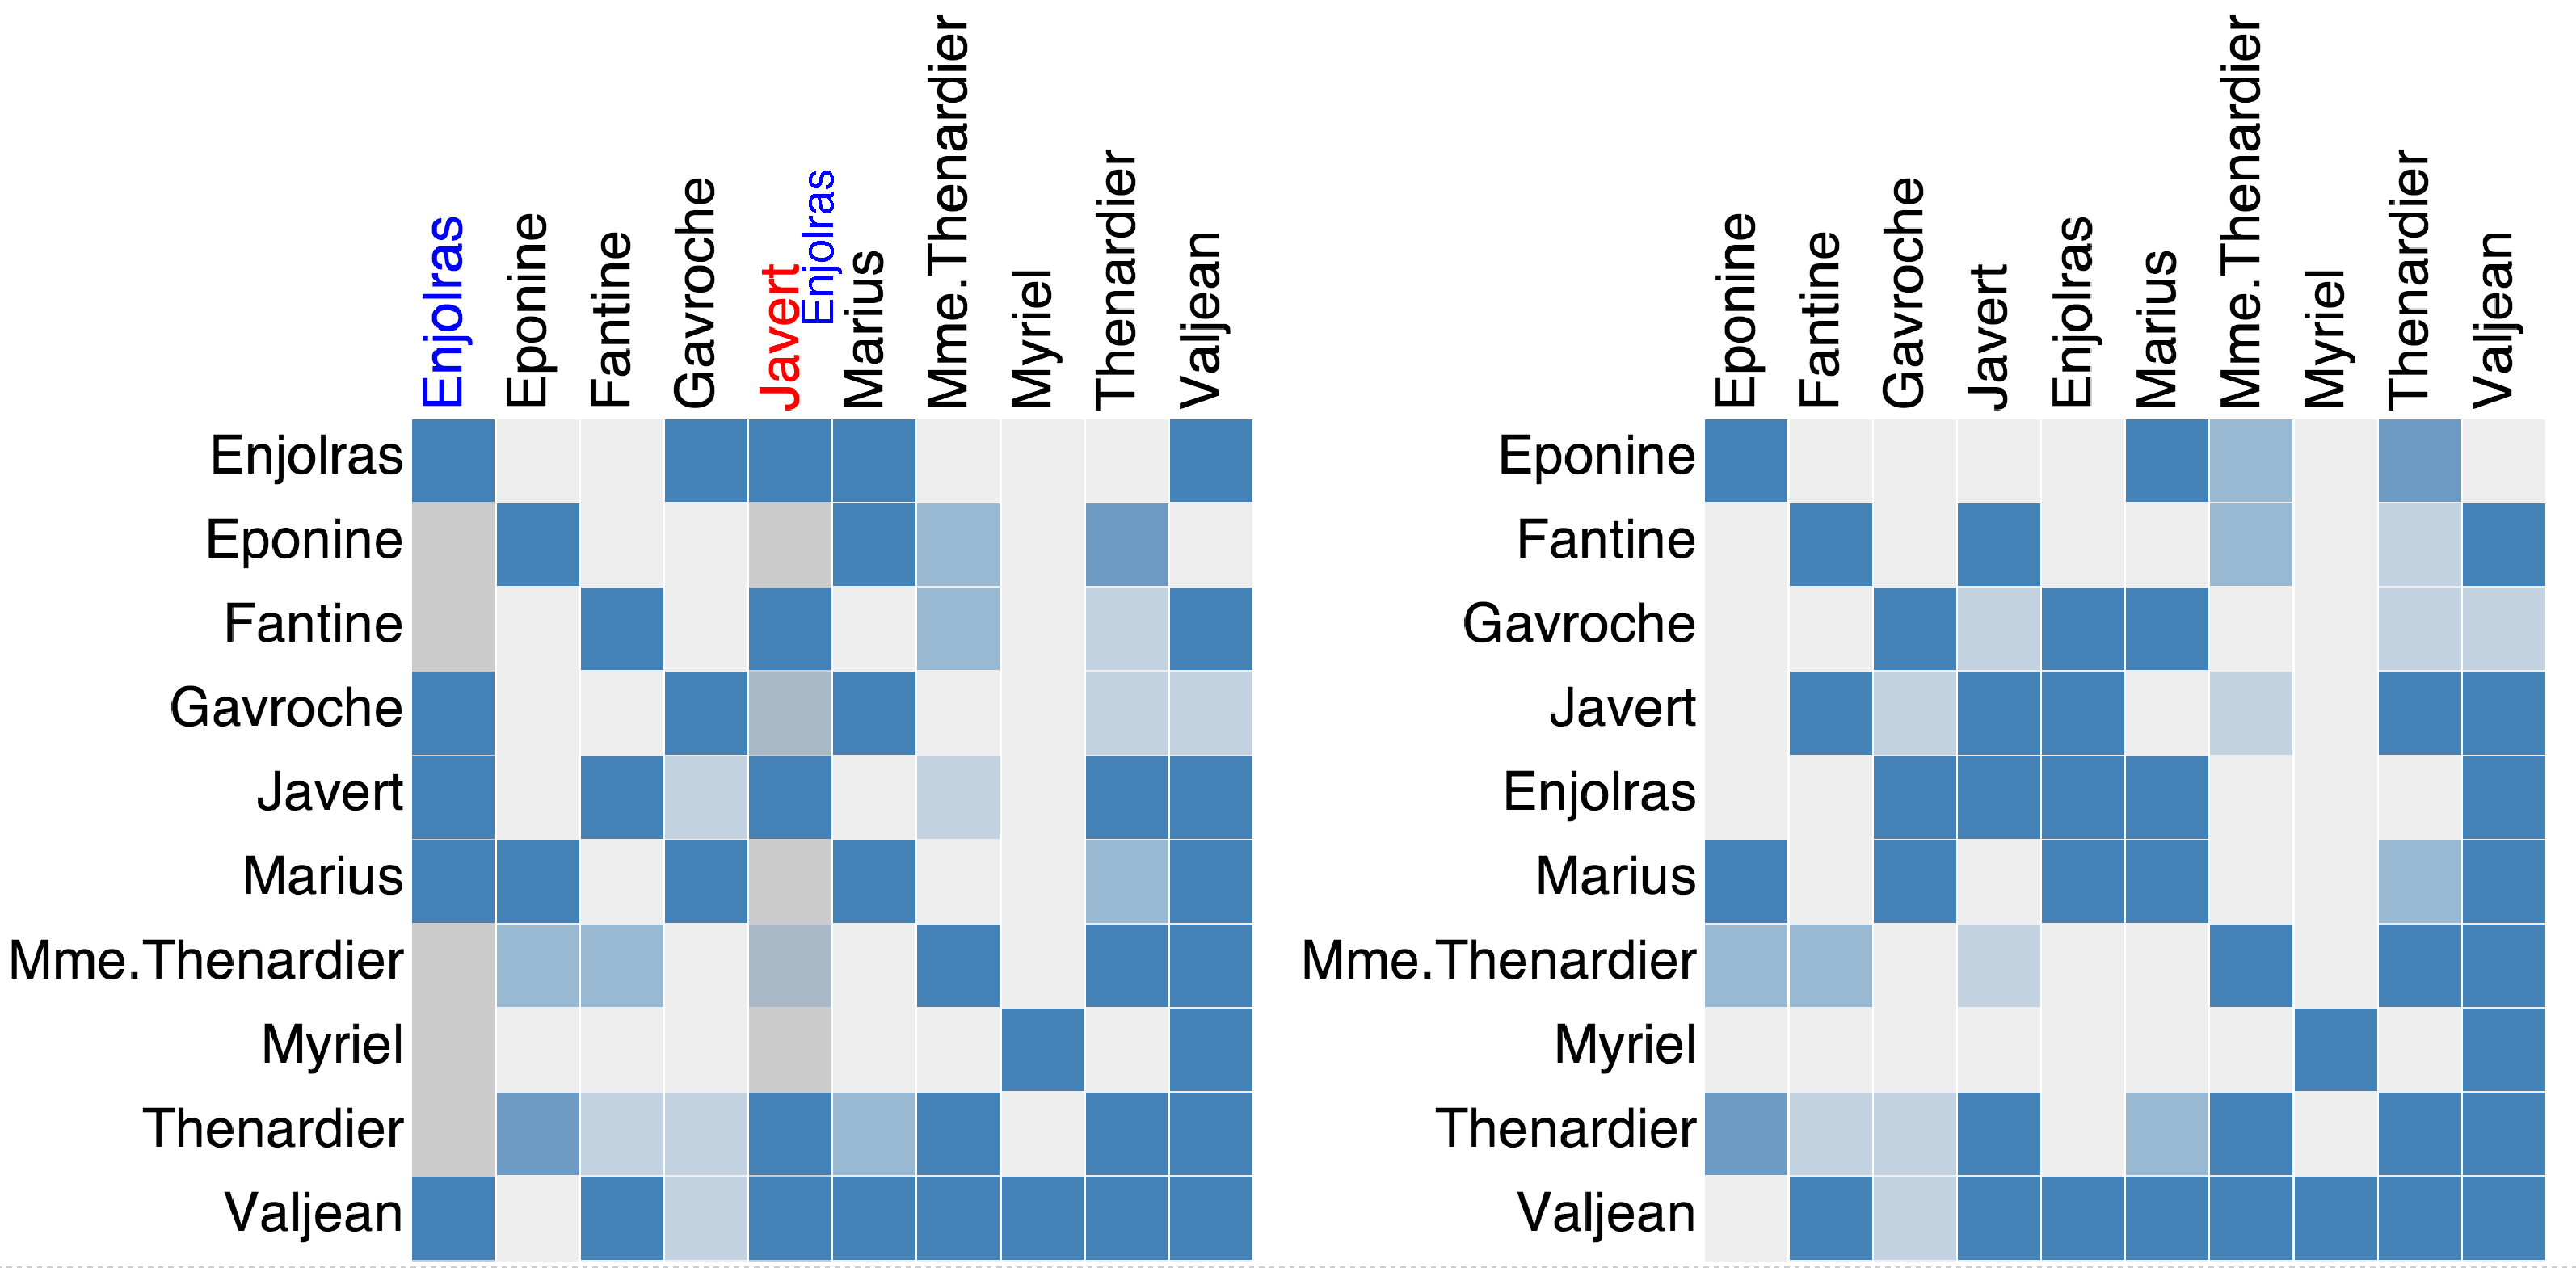
\includegraphics
  [width=0.6\textwidth]{cooccurrence}}
\end{wrapfigure}

\vspace{-7pt}

The figure to the left shows a co-occurrence matrix of Les Mis\'{e}rables
characters. To reorder the columns of the matrix, we first construct a data
source that computes the sort order of characters and initialize it to an
alphabetical ordering. A signal on \texttt{@col\_label:mousedown} captures the
source column to be reordered, while a signal on \texttt{[@col\_label:mousedown,
mouseup] > mousemove} updates the target column location. On \texttt{mouseup},
the data source is updated to swap the two sorting indices.

\vspace{-10pt}

\subsection{Filter: Control Widgets}

\vspace{-7pt}

\begin{figure}[t!]
  \centering
  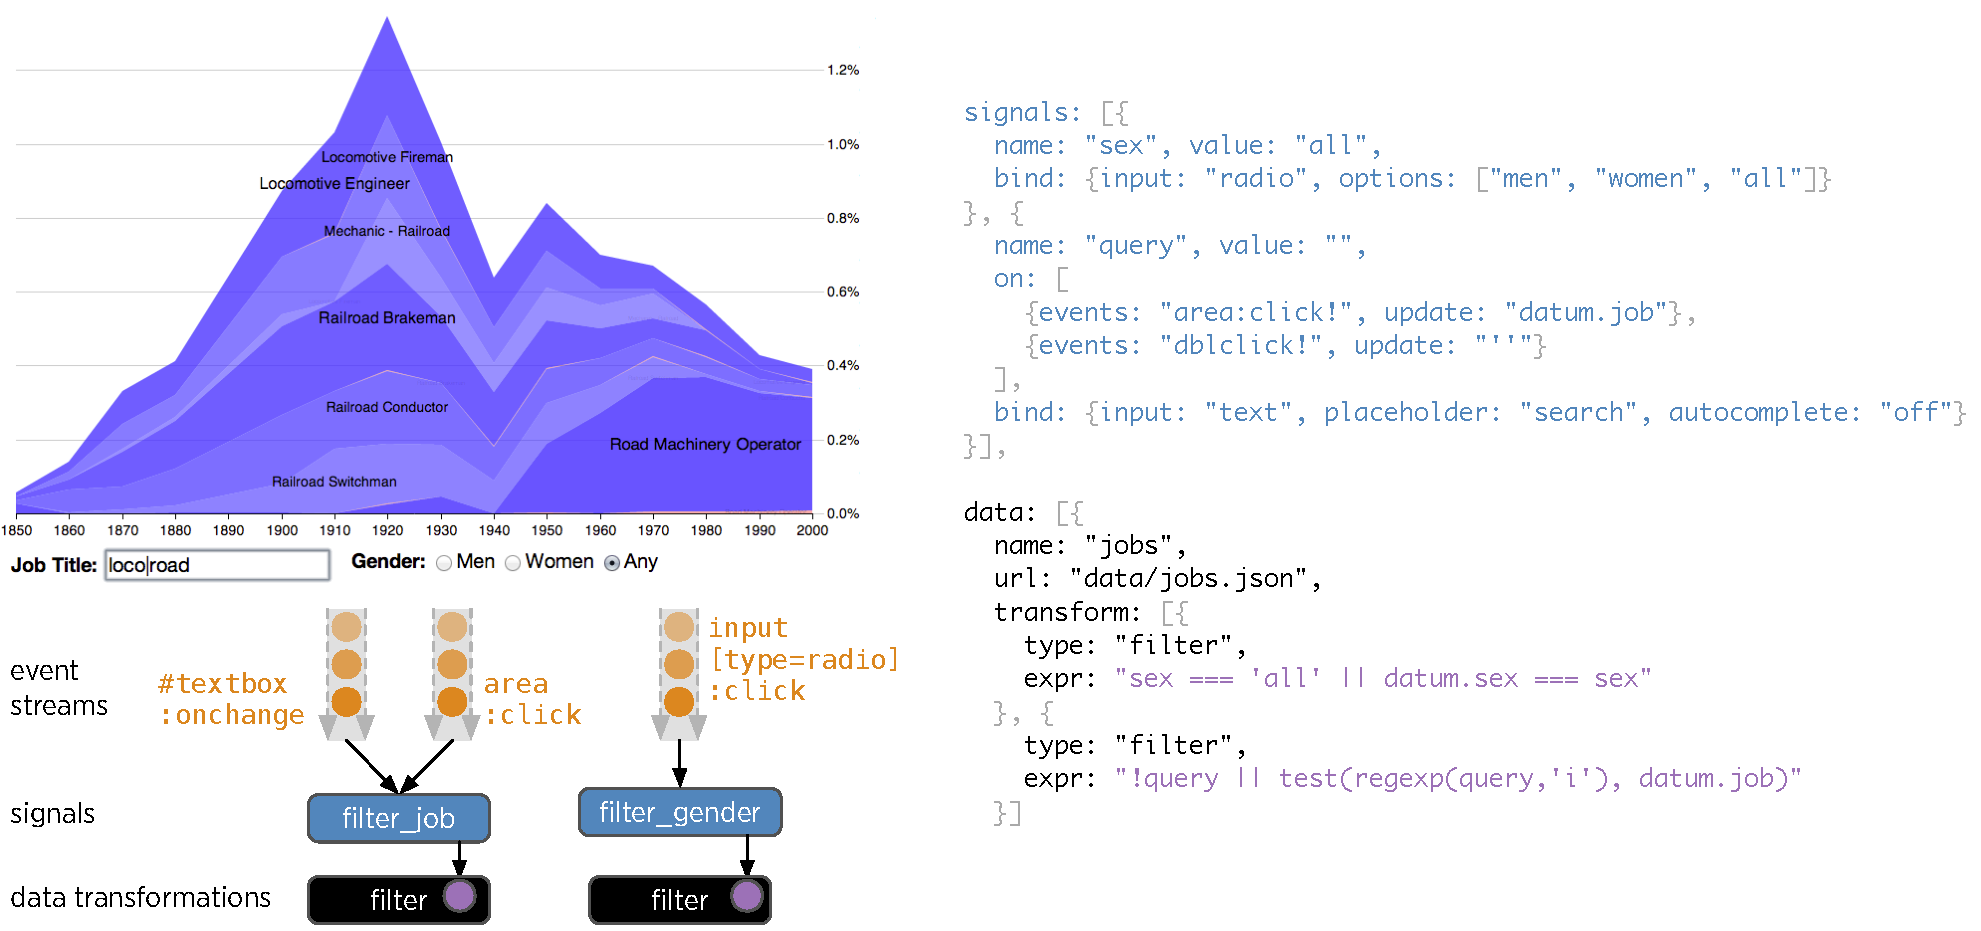
\includegraphics[width=0.9\columnwidth]{jobVoyager}
  \caption{The job voyager can be filtered using signals bound to control
  widgets. The textbox pattern matches against job titles while radio buttons
  filter by gender.}
  \label{fig:vg:jobVoyager}
\end{figure}

\Cref{fig:vg:jobVoyager} shows the Job Voyager~\cite{heer:voyagers}
visualization with control widgets to filter the visualized data. A textbox
allows users to enter search terms to filter job titles, while the radio buttons
allow users to filter by gender. We bind signals to the value of these control
widgets, and then construct predicates attached to filter data transformations.
For the textbox signal, a regular expression tests terms against job titles,
while an equality test filters by gender based on the radio button signal. This
example illustrates how external widgets can easily be bound to our reactive
model.

\vspace{-20pt}

\subsection{DimpVis: Touch Navigation with Time-Series Data}

\vspace{-7pt}

DimpVis~\cite{kondo:dimpvis} is a recently introduced interaction technique that
allows direct manipulation navigation of time-series data. Starting with a
scatterplot depicting data at a particular time slice, users can touch plotted
points to reveal a ``hint path'': a line graph that displays the trajectory of
the selected element over time. Dragging the selected point along this path
triggers temporal navigation, with the rest of the points updating to reflect
the new time. In evaluation studies, users reported feeling more engaged when
exploring their data using DimpVis~\cite{kondo:dimpvis}.

As shown in \cref{fig:vg:dimpvis}, we can recreate this technique with Reactive
Vega's declarative interaction primitives and the GapMinder
country-fertility-life-expectancy dataset used by the original. Input data is
passed through a \texttt{Window} transform, such that every tuple contains
references to the tuples that come before and after it in time, and filtered to
remove triplets that span multiple countries. Signals constructed over mouse and
touch events capture the selected point, and downstream signals calculate
distances between the user's current position and the previous and next points.
A scalar projection over these distances gives us scoring functions that
determine whether the user is moving forwards or backwards in time. Scores feed
a signal that is used in a derived data source to calculate new interpolated
properties for the remaining points in the dataset. These interpolated
properties determine the position of plotted points, producing smooth
transitions as the user drags back-and-forth. To draw the hint map, a derived
data source filters data tuples for the selected country across all years.

\begin{figure}[h!]
  \centering
  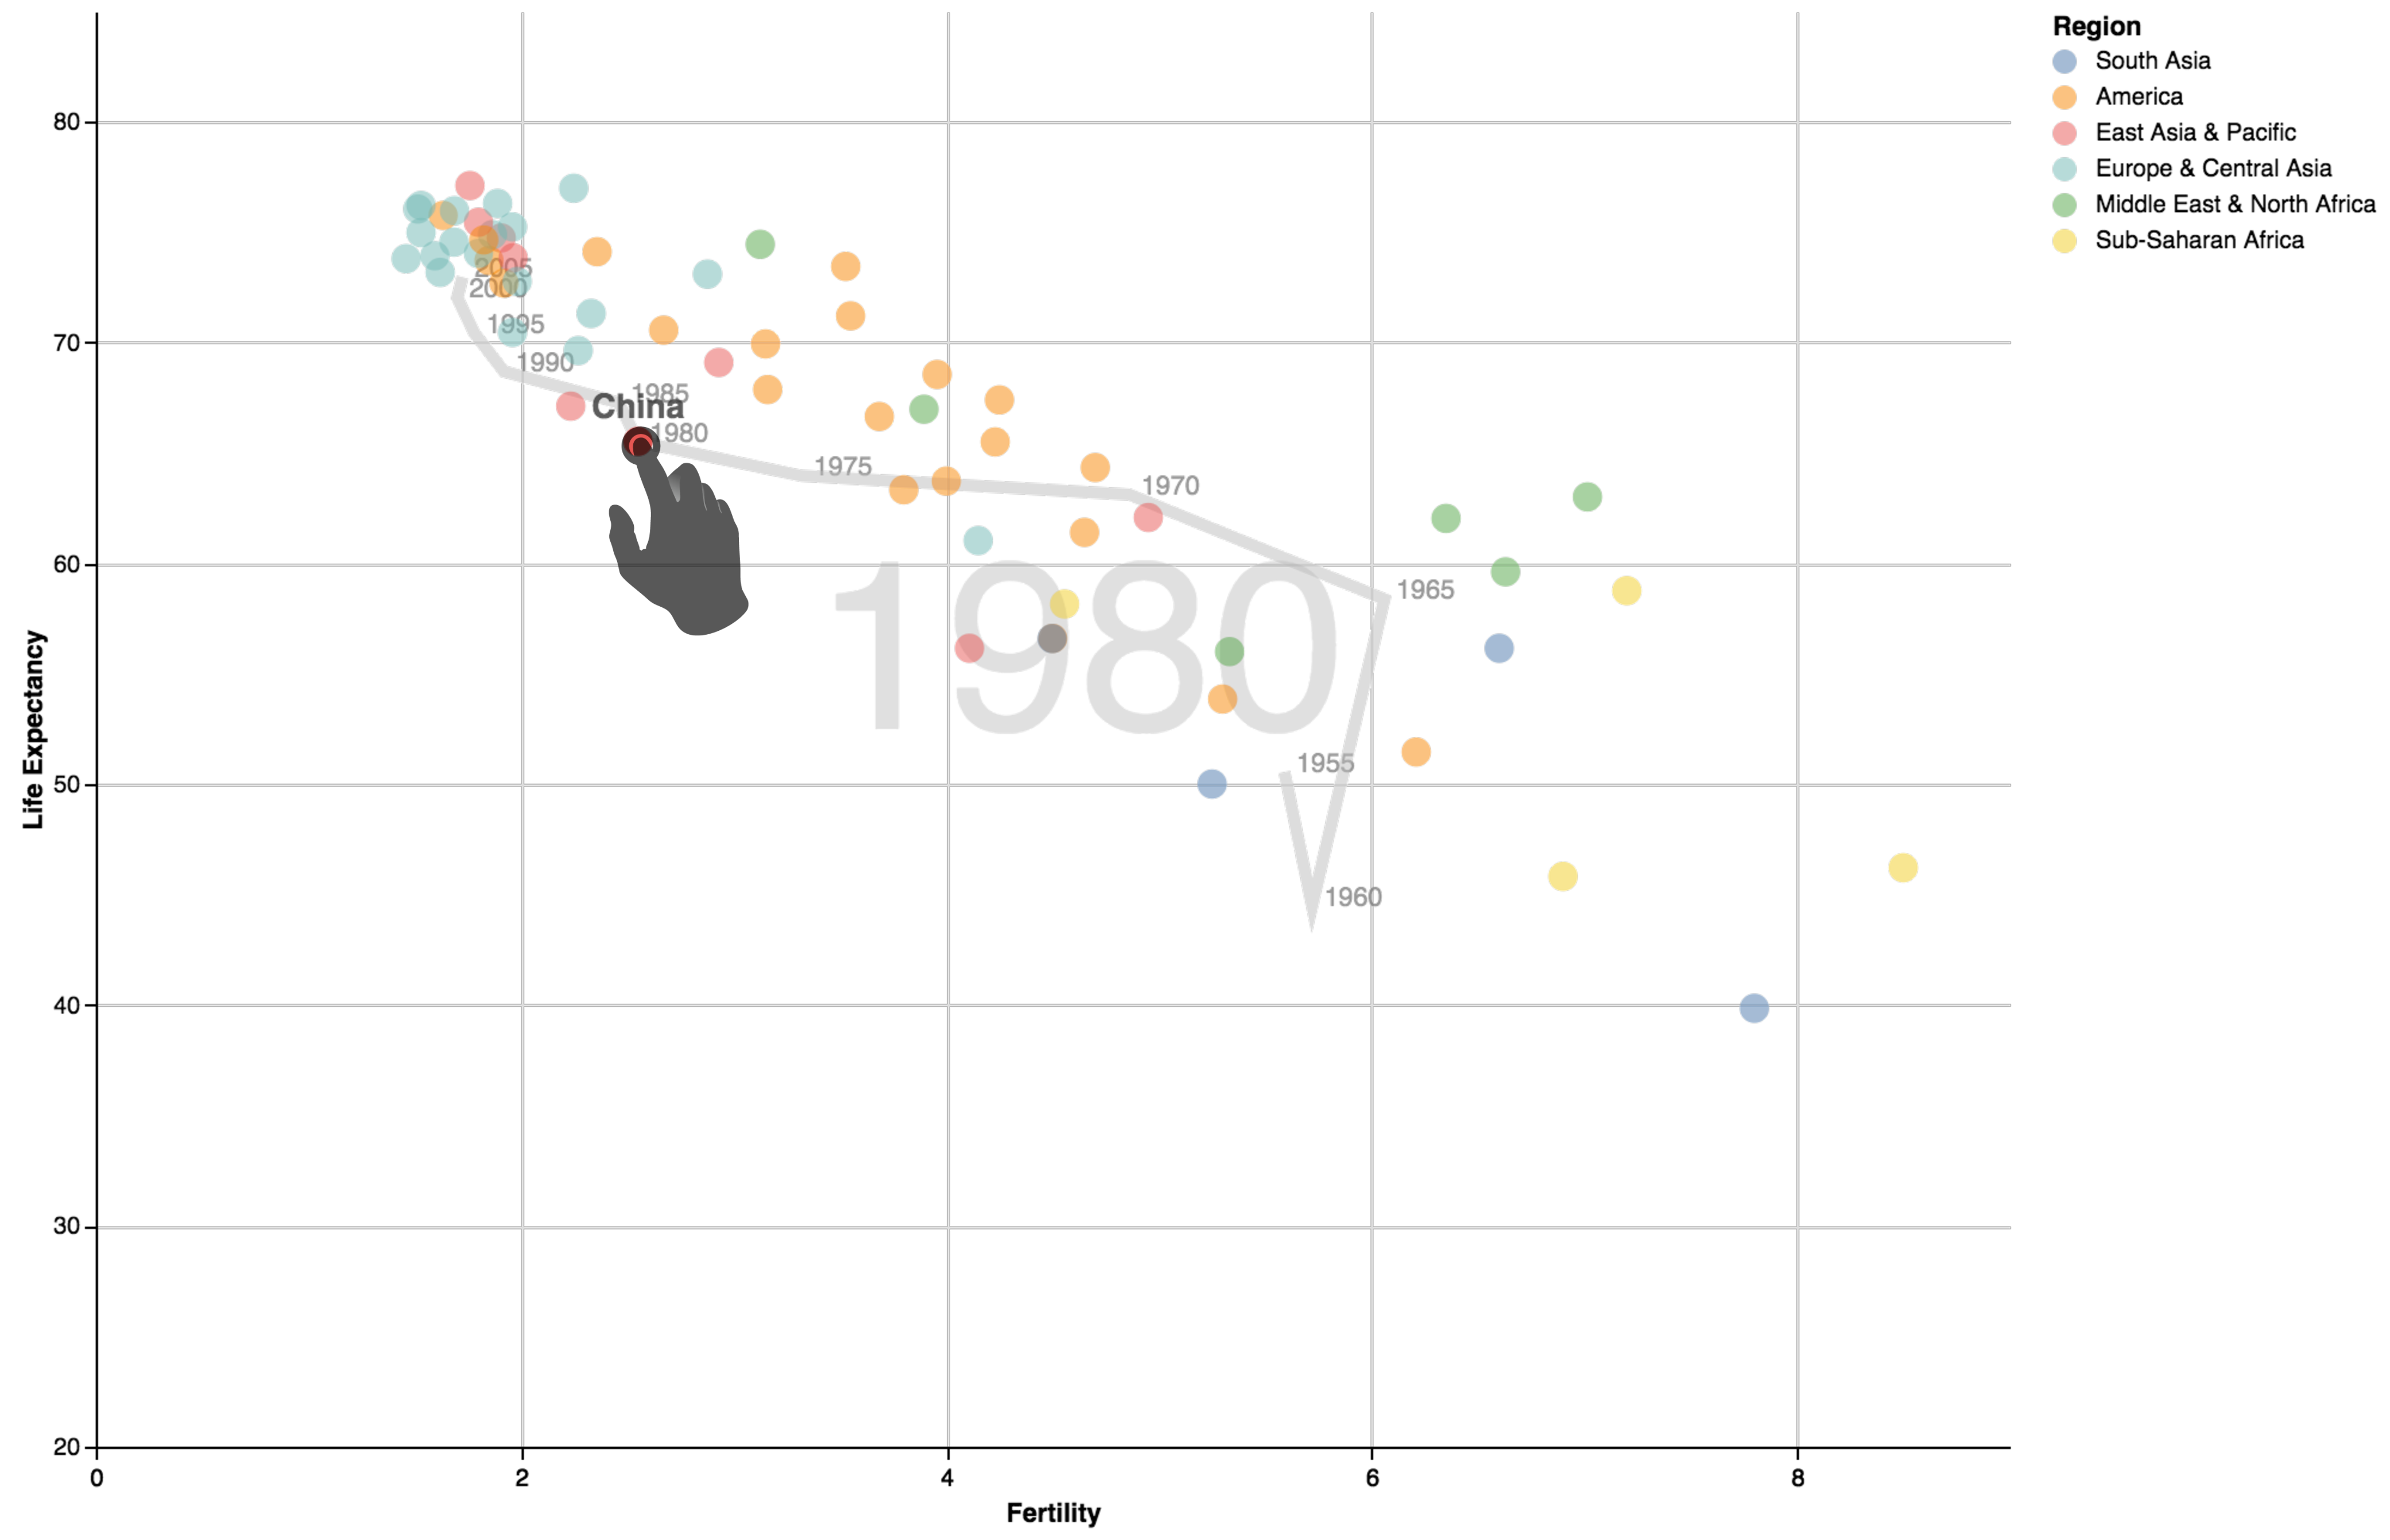
\includegraphics[width=\columnwidth]{dimpvis}
  \caption{DimpVis~\cite{kondo:dimpvis}, touch-based navigation of time-series
  data recreated with Reactive Vega.}
  \label{fig:vg:dimpvis}
\end{figure}

\vspace{-10pt}

\subsection{Reusable Touch Interaction Abstractions}

\vspace{-7pt}

With the proliferation of touch-enabled devices, particularly smartphones and
tablets, supporting touch-based interaction has become an increasingly important
part of interactive visualization design. However, HTML5 only provides a
low-level API for touch events, with three event types broadly
supported\,---\,\texttt{touchstart}, \texttt{touchmove}, and \texttt{touchend}.
On multitouch devices these events contain an array of touch points. The
application developer is responsible for the bookkeeping involved with tracking
multiple points across interactions, a cumbersome and difficult process.

Declarative interaction design enables us to abstract low-level details away,
building reusable interactors that expose higher-level, semantic events as
signals instead. For example, an interactor could define signals that perform
the necessary logic for common multitouch gestures. Once such an interactor is
included in a host visualization, the visualization designer can then safely
ignore lower-level events, and instead build interactions driven by the
interactor's signals\,---\,using \texttt{twotouchmove} and \texttt{pinchDelta}
signals to drive panning and zooming behaviors, for instance.